En este capítulo hablaremos de algunas herramientas y paquetes de Python que existen actualmente para garantizar la equidad en aprendizaje automático. Hablaremos de algunos de los más influyentes, entre los que destacaremos Aequitas. 

\section{Paquetes de Python para equidad en AA}

\section*{Ethik}

Ethik es un paquete de Python para realizar estudios sobre equidad en aprendizaje automático y obtener explicaciones sobre la misma. Ethik utiliza el enfoque de la equidad contrafactual para dar solución a escenarios hipotéticos de injusticia en una población concreta. El paquete contiene una recopilación de conjuntos de datos sobre problemas de equidad a partir de la cual hemos podido extraer el \textit{dataset} denominado \textit{law\_data.csv}, que contiene el problema del Apartado \ref{subsec:desproblem}, usando la función \texttt{load\_law\_school()}.

Podemos encontrar la documentación y herramientas que proporciona el paquete en el \href{https://xai-aniti.github.io/ethik/}{siguiente enlace}\footnote{https://xai-aniti.github.io/ethik/}.

\section*{Fairlearn}

Fairlearn es un paquete de Python que permite a los científicos de datos y desarrolladores de aplicaciones de \textit{machine learning} evaluar la equidad de su sistema, y mitigar cualquier problema de sesgo en una población para un conjunto de datos observado. Fairlearn contiene  algoritmos de mitigación, así como métricas para la evaluación del modelo.

Podemos encontrar la documentación y una guía de uso del paquete en el \href{https://fairlearn.org/v0.5.0/user_guide/index.html}{siguiente enlace}\footnote{https://fairlearn.org/v0.5.0/user\_guide/index.html}.

\section{Aequitas}

Aequitas (\cite{aequitas2019}) es una herramienta de auditoría desarrollada por el \textit{Center for Data Science and Public Policy} de la
Universidad de Chicago. Es una herramienta de código abierto que consta de diversas utilidades de soporte para la auditoría de sesgos; creado para ser utilizado por analistas de todo tipo relacionados con el ámbito del aprendizaje automático, y cuyo principal objetivo es auditar los modelos de \textit{machine learning}, con el fin de encontrar posibles discriminaciones en ellos y evitarlas en un futuro.

Aequitas nos permite detectar dos tipos de sesgos:

\begin{itemize}
    \item Acciones sesgadas que no ocurren de forma representativa en la población.
    \item Resultados sesgados, a causa de errores de clasificación de nuestro sistema, con respecto a ciertos grupos de la población.
\end{itemize}

Para utilizar la herramienta se necesita aportar los siguientes datos:

\begin{itemize}
    \item Datos sobre los atributos específicos (raza, sexo, etc.) que queramos auditar.
    \item El conjunto de personas de la población mencionada que el sistema de evaluación de riesgos seleccionó para una intervención.
\end{itemize}

\subsection*{Estructura de los datos de entrada y resultados}

Podemos dividir en tres apartados (conformados por columnas en Aequitas) los datos que debemos aportar para el correcto funcionamiento de la herramienta.

\begin{itemize}
    \item \textbf{score}: representa la conclusión a la que llega un modelo, puede ser binaria ($0$ o $1$) o continua (decimal entre $0$ y $1$). Esta decisión representa si el sujeto es apto o no, por ejemplo, si se le concede un crédito bancario.
    \item \textbf{label\_value}: representa los datos reales; es decir, si la predicción realizada por el modelo fue correcta. Por ejemplo, el sujeto fue capaz de devolver el crédito en su totalidad. Es por esto por lo que el modelo solo puede ser auditado después de su aplicación y no antes. Se representa como un valor binario, $1$ significa que la predicción fue correcta, $0$ que no lo fue.
    \item \textbf{attributes}: categorías de los atributos definidos por el usuario y utilizados para decidir la equidad del modelo. Algunos ejemplos de atributos son la raza, sexo, educación, edad o ingresos.
\end{itemize}

El funcionamiento de Aequitas viene determinado por los conceptos y métricas definidas previamente en la Sección \ref{sec:groupmetrics}. Podemos acceder a una lista de los conceptos y métricas que utiliza Aequitas desde el \href{https://dssg.github.io/aequitas/metrics.html}{siguiente enlace}\footnote{https://dssg.github.io/aequitas/metrics.html}.

La herramienta devuelve una interpretación gráfica de los resultados junto a información relevante acerca de tres tipos de métricas:

\begin{itemize}
    \item \textbf{Métricas de grupo -} Los grupos podrán definirse utilizando la clase \textit{Group()}.
    \item \textbf{Métricas de disparidad -} Las disparidades podrán ser calculadas haciendo uso de la clase \textit{Bias()}, una vez calculadas las métricas de grupo.
    \item \textbf{Medidas de equidad -} Estudiaremos la equidad y gráficos de distribución de las métricas de grupo y disparidad a partir de la clase \textit{Fairness()}.
\end{itemize}

A continuación mostraremos dos ejemplos de uso de Aequitas haciendo uso de las diferentes alternativas que ofrece para auditar un \textit{dataset}. Por un lado, usaremos la herramienta WEB para analizar la información acerca de las medidas de equidad ofrecidas, y por otro la API de Python que incluye un mayor número de métricas y gráficas para interpretar los resultados.

\subsection{Ejemplo: Puntuación del riesgo de reincidencia delictiva}

En este apartado, analizaremos cómo se definen las diferentes métricas con las que trabaja Aequitas a partir de los conceptos previamente estudiados. Mostraremos un ejemplo sobre el conjunto de datos \textit{COMPAS}, cuyo objetivo era identificar a las personas con riesgo de reincidencia, para respaldar las decisiones de liberación previa al juicio.\\

\begin{table}[h]
\centering
\resizebox{12.4cm}{!} {
\begin{tabular}{|c|c|c|c|c|}
\hline
\textbf{score} & \textbf{label\_value} & \textbf{race}    & \textbf{sex} & \textbf{age\_cat} \\ \hline
1            & 0                     & Hispanic & Male       & Less than 25             \\ \hline
0              & 1                     & African-American         & Female         & 25-45     \\ \hline
0              & 0                     & Caucasian       & Male         & Greater than 45            \\ \hline
\end{tabular}
}
\caption{Ejemplo del \textit{dataset COMPAS} aportado a Aequitas.}
\label{tab:ejcompasaeq}
\end{table}

Los datos están basados en las estadísticas recogidas en el condado de Broward y puestas a disposición del público por la organización ProPublica (\cite{condena2016}). Este conjunto de datos contiene una puntuación del riesgo de reincidencia para 7.214 individuos, sus resultados reales de reincidencia a los dos años, y una serie de atributos recogidos entre 2013 y 2014. Para tratar la puntuación de riesgo con Aequitas, convertiremos el \textit{score} original (1-10) a uno binario donde 0 indica riesgo bajo y 1 medio o alto.

\subsection*{Análisis de los datos}

En los gráficos siguientes podemos notar una gran diferencia en la distribución de las puntuaciones por raza (Figura \ref{fig:barrasrace}), con una mayoría de personas de raza caucásica pronosticadas como riesgo bajo (\textit{score}=0) y una mayoría de población afroamericana pronosticada como riesgo medio o alto (\textit{score}=1). En cuanto al atributo edad (Figura \ref{fig:barrasage}), se predicen como riesgo bajo la mayoría de las personas de edad superior a 25 años y como riesgo medio-alto a la mayoría de los menores de 25 años. Finalmente, aunque existen muchos más hombres que mujeres en la base de datos (los hombres tienen un índice de criminalidad mayor que las mujeres); parece que, en principio, el sexo (Figura \ref{fig:barrassex}) no es determinante a la hora de puntuar la reincidencia.

Además, incluimos gráficos de cómo se distribuyen las etiquetas reales según los atributos protegidos. Las etiquetas reales contienen la información sobre si el sujeto reincidió (\textit{label\_value}=1) o no (\textit{label\_value}=0); es decir, si el individuo sufrió una nueva detención en un plazo de dos años. Con esta información podremos comprobar directamente la precisión de las predicciones.\\

\begin{figure}[h]
    \minipage{0.53\textwidth}
      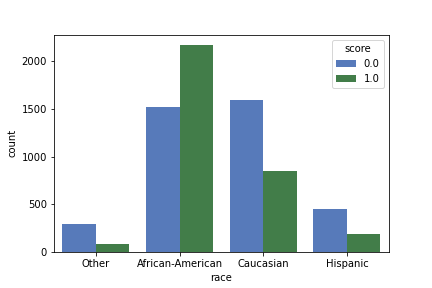
\includegraphics[width=\linewidth]{images/score_race.png}
    \endminipage\hfill
    \minipage{0.53\textwidth}%
      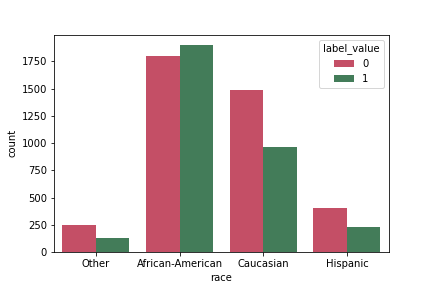
\includegraphics[width=\linewidth]{images/label_race.png}
    \endminipage
     \caption{Gráfico de barras de la puntuación y etiqueta real para el atributo \textit{race}.}
     \label{fig:barrasrace}
\end{figure}

\begin{figure}[h]
    \minipage{0.53\textwidth}
      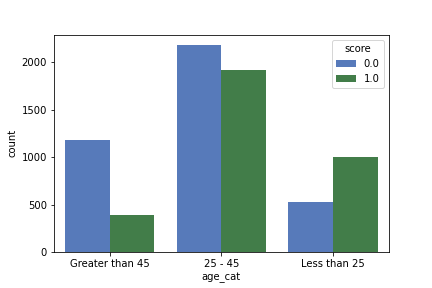
\includegraphics[width=\linewidth]{images/score_age.png}
    \endminipage\hfill
    \minipage{0.53\textwidth}%
      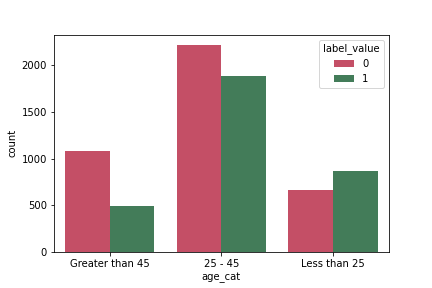
\includegraphics[width=\linewidth]{images/label_age.png}
    \endminipage
     \caption{Gráfico de barras de la puntuación y etiqueta real para el atributo \textit{age\_cat}.}
     \label{fig:barrasage}
\end{figure}

\begin{figure}[h]
    \minipage{0.53\textwidth}
      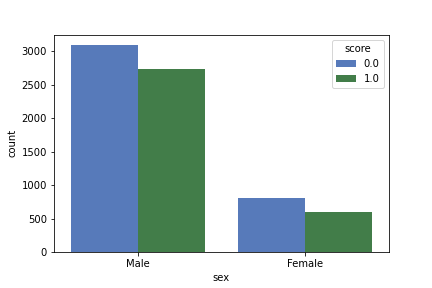
\includegraphics[width=\linewidth]{images/score_sex.png}
    \endminipage\hfill
    \minipage{0.53\textwidth}%
      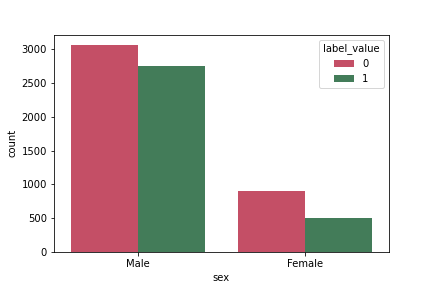
\includegraphics[width=\linewidth]{images/label_sex.png}
    \endminipage
     \caption{Gráfico de barras de la puntuación y etiqueta real para el atributo \textit{sex}.}
     \label{fig:barrassex}
\end{figure}

En la Figura \ref{fig:barrasrace} podemos observar que donde se detecta una mayor diferencia entre las gráficas de puntuación de riesgo y la reincidencia real, es en el grupo de los individuos de raza afroamericana. Este hecho induce a preguntarnos si estos patrones podrían reflejar o no un sesgo en la población, que fuese perjudicial a la hora de utilizar \textit{COMPAS} como un conjunto de datos de entrenamiento para un modelo de aprendizaje automático.

Utilizaremos la herramienta de Aequitas para realizar un estudio de los posibles patrones de sesgo que pudiesen existir entre los diferentes grupos de la población que representa el conjunto de datos \textit{COMPAS}.

\subsection*{Métricas de grupo}

Haciendo uso de la clase \textit{Group()}, calcularemos una tabla con los valores de las métricas de grupo para un atributo concreto (p.ej. raza).

\begin{table}[h]
\centering
\resizebox{12.6cm}{!} {
\begin{tabular}{cccccccc}
{\color[HTML]{3166FF} race}                                                              & \multicolumn{1}{l}{}                                                                     & \multicolumn{1}{l}{}                             & \multicolumn{1}{l}{}                             & \multicolumn{1}{l}{}                             & \multicolumn{1}{l}{}                             & \multicolumn{1}{l}{}                             & \multicolumn{1}{l}{}                             \\
{\color[HTML]{3166FF} }                                                                  & \multicolumn{1}{l}{}                                                                     & \multicolumn{1}{l}{}                             & \multicolumn{1}{l}{}                             & \multicolumn{1}{l}{}                             & \multicolumn{1}{l}{}                             & \multicolumn{1}{l}{}                             & \multicolumn{1}{l}{}                             \\ \hline
\multicolumn{1}{|c|}{\textbf{\begin{tabular}[c]{@{}c@{}}Attribute\\ Value\end{tabular}}} & \multicolumn{1}{c|}{\textbf{\begin{tabular}[c]{@{}c@{}}Group Size\\ Ratio\end{tabular}}} & \multicolumn{1}{c|}{\textbf{PPR}}                & \multicolumn{1}{c|}{\textbf{PPREV}}              & \multicolumn{1}{c|}{\textbf{FDR}}                & \multicolumn{1}{c|}{\textbf{FPR}}                & \multicolumn{1}{c|}{\textbf{FOR}}                & \multicolumn{1}{c|}{\textbf{FNR}}                \\ \hline
\multicolumn{1}{|c|}{\begin{tabular}[c]{@{}c@{}}African-\\ American\end{tabular}}        & \multicolumn{1}{c|}{0.51}                                                                & \multicolumn{1}{c|}{{0.66}} & \multicolumn{1}{c|}{{0.59}} & \multicolumn{1}{c|}{{0.37}} & \multicolumn{1}{c|}{{0.45}} & \multicolumn{1}{c|}{{0.35}} & \multicolumn{1}{c|}{{0.28}} \\ \hline
\multicolumn{1}{|c|}{Asian}                                                              & \multicolumn{1}{c|}{0}                                                                   & \multicolumn{1}{c|}{{0.0}}  & \multicolumn{1}{c|}{{ 0.25}} & \multicolumn{1}{c|}{{ 0.25}} & \multicolumn{1}{c|}{{0.09}} & \multicolumn{1}{c|}{{ 0.12}} & \multicolumn{1}{c|}{{0.33}} \\ \hline
\multicolumn{1}{|c|}{Caucasian}                                                          & \multicolumn{1}{c|}{0.34}                                                                & \multicolumn{1}{c|}{0.26}                        & \multicolumn{1}{c|}{0.35}                        & \multicolumn{1}{c|}{0.41}                        & \multicolumn{1}{c|}{0.23}                        & \multicolumn{1}{c|}{0.29}                        & \multicolumn{1}{c|}{0.48}                        \\ \hline
\multicolumn{1}{|c|}{Hispanic}                                                           & \multicolumn{1}{c|}{0.09}                                                                & \multicolumn{1}{c|}{{0.06}} & \multicolumn{1}{c|}{{ 0.3}}  & \multicolumn{1}{c|}{{ 0.46}} & \multicolumn{1}{c|}{{ 0.21}} & \multicolumn{1}{c|}{{ 0.29}} & \multicolumn{1}{c|}{{ 0.56}} \\ \hline
\multicolumn{1}{|c|}{\begin{tabular}[c]{@{}c@{}}Native\\ American\end{tabular}}          & \multicolumn{1}{c|}{0}                                                                   & \multicolumn{1}{c|}{{ 0.0}}  & \multicolumn{1}{c|}{{ 0.67}} & \multicolumn{1}{c|}{{ 0.25}} & \multicolumn{1}{c|}{{ 0.38}} & \multicolumn{1}{c|}{{ 0.17}} & \multicolumn{1}{c|}{{ 0.1}}  \\ \hline
\multicolumn{1}{|c|}{Other}                                                              & \multicolumn{1}{c|}{0.05}                                                                & \multicolumn{1}{c|}{{ 0.02}} & \multicolumn{1}{c|}{{ 0.21}} & \multicolumn{1}{c|}{{ 0.46}} & \multicolumn{1}{c|}{{ 0.15}} & \multicolumn{1}{c|}{{ 0.3}}  & \multicolumn{1}{c|}{{ 0.68}} \\ \hline
\end{tabular}
}
	\caption{Tabla con las principales métricas de grupo para el atributo \textit{race}.}
    \label{fig:ejaq1}
\end{table}

\subsection*{Métricas de disparidad}

Tomaremos como atributo de referencia la raza \textit{Caucasian}. En nuestro caso la raza \textit{Caucasian} no es la raza mayoritaria en el conjunto de datos, pero la tomaremos como referencia debido a que históricamente en el ámbito en el que nos movemos es la que sufre menos sesgos.

A continuación usaremos la clase \textit{Bias()} para medir la disparidad entre cada grupo objetivo y el grupo de referencia seleccionado. Aequitas calcula la disparidad a partir de la fórmula que ya definimos en el Apartado \ref{subsec:impactdesi}. $$\text{Métrica de disparidad}_{G(a_o)}=\ddfrac{\text{Métrica}_{a_o}}{\text{Métrica}_{a_r}},$$ donde Métrica hace referencia a una métrica de grupo de la Sección \ref{sec:groupmetrics}. Es evidente que la disparidad de cualquier métrica sobre el grupo de referencia será 1. $$\text{Métrica de disparidad}_{G(a_r)}=\ddfrac{\text{Métrica}_{a_r}}{\text{Métrica}_{a_r}}=1.$$

Si queremos calcular por ejemplo la disparidad del ratio de falsos negativos (FNR) sobre el grupo de raza \textit{Asian}, se calculará de la siguiente forma: $$\text{FNR}_{\text{G(Asian)}}=\ddfrac{\text{FNR}_{\text{Asian}}}{\text{FNR}_{\text{Caucasian}}}=\ddfrac{0.33}{0.48}=0.7.$$

Para ver otro ejemplo de cómo realiza el cálculo Aequitas, mediremos la disparidad para la tasa de falso descubrimiento (FDR) sobre el grupo de raza \textit{Hispanic}:
$$\text{FDR}_{\text{G(Hispanic)}}=\ddfrac{\text{FDR}_{\text{Hispanic}}}{\text{FDR}_{\text{Caucasian}}}=\ddfrac{0.46}{0.41}=1.12.$$

Completando la tabla con las métricas de disparidad para todas las métricas de grupo obtendremos el siguiente resultado:

\begin{table}[h]
\centering
\resizebox{14.cm}{!} {
\begin{tabular}{ccccccc}
{\color[HTML]{3166FF} race}                                                              & \multicolumn{1}{l}{}                                                                  & \multicolumn{1}{l}{}                                                                    & \multicolumn{1}{l}{}                                                                  & \multicolumn{1}{l}{}                                                                  & \multicolumn{1}{l}{}                                                                  & \multicolumn{1}{l}{}                                                                  \\
{\color[HTML]{3166FF} }                                                                  & \multicolumn{1}{l}{}                                                                  & \multicolumn{1}{l}{}                                                                    & \multicolumn{1}{l}{}                                                                  & \multicolumn{1}{l}{}                                                                  & \multicolumn{1}{l}{}                                                                  & \multicolumn{1}{l}{}                                                                  \\ \hline
\multicolumn{1}{|c|}{\textbf{\begin{tabular}[c]{@{}c@{}}Attribute\\ Value\end{tabular}}} & \multicolumn{1}{c|}{\textbf{\begin{tabular}[c]{@{}c@{}}PPR\\ Disparity\end{tabular}}} & \multicolumn{1}{c|}{\textbf{\begin{tabular}[c]{@{}c@{}}PPREV\\ Disparity\end{tabular}}} & \multicolumn{1}{c|}{\textbf{\begin{tabular}[c]{@{}c@{}}FDR\\ Disparity\end{tabular}}} & \multicolumn{1}{c|}{\textbf{\begin{tabular}[c]{@{}c@{}}FPR\\ Disparity\end{tabular}}} & \multicolumn{1}{c|}{\textbf{\begin{tabular}[c]{@{}c@{}}FOR\\ Disparity\end{tabular}}} & \multicolumn{1}{c|}{\textbf{\begin{tabular}[c]{@{}c@{}}FNR\\ Disparity\end{tabular}}} \\ \hline
\multicolumn{1}{|c|}{\begin{tabular}[c]{@{}c@{}}African-\\ American\end{tabular}}        & \multicolumn{1}{c|}{{\color[HTML]{FE0000} 2.55}}                                      & \multicolumn{1}{c|}{{\color[HTML]{FE0000} 1.69}}                                        & \multicolumn{1}{c|}{{\color[HTML]{32CB00} 0.91}}                                      & \multicolumn{1}{c|}{{\color[HTML]{FE0000} 1.91}}                                      & \multicolumn{1}{c|}{{\color[HTML]{32CB00} 1.21}}                                      & \multicolumn{1}{c|}{{\color[HTML]{FE0000} 0.59}}                                      \\ \hline
\multicolumn{1}{|c|}{Asian}                                                              & \multicolumn{1}{c|}{{\color[HTML]{FE0000} 0.01}}                                      & \multicolumn{1}{c|}{{\color[HTML]{FE0000} 0.72}}                                        & \multicolumn{1}{c|}{{\color[HTML]{FE0000} 0.61}}                                      & \multicolumn{1}{c|}{{\color[HTML]{FE0000} 0.37}}                                      & \multicolumn{1}{c|}{{\color[HTML]{FE0000} 0.43}}                                      & \multicolumn{1}{c|}{{\color[HTML]{FE0000} 0.7}}                                       \\ \hline
\multicolumn{1}{|c|}{Caucasian}                                                          & \multicolumn{1}{c|}{{\color[HTML]{3166FF} 1.0}}                                       & \multicolumn{1}{c|}{{\color[HTML]{3166FF} 1.0}}                                         & \multicolumn{1}{c|}{{\color[HTML]{3166FF} 1.0}}                                       & \multicolumn{1}{c|}{{\color[HTML]{3166FF} 1.0}}                                       & \multicolumn{1}{c|}{{\color[HTML]{3166FF} 1.0}}                                       & \multicolumn{1}{c|}{{\color[HTML]{3166FF} 1.0}}                                       \\ \hline
\multicolumn{1}{|c|}{Hispanic}                                                           & \multicolumn{1}{c|}{{\color[HTML]{FE0000} 0.22}}                                      & \multicolumn{1}{c|}{{\color[HTML]{32CB00} 0.86}}                                        & \multicolumn{1}{c|}{{\color[HTML]{32CB00} 1.12}}                                      & \multicolumn{1}{c|}{{\color[HTML]{32CB00} 0.92}}                                      & \multicolumn{1}{c|}{{\color[HTML]{32CB00} 1.0}}                                       & \multicolumn{1}{c|}{{\color[HTML]{32CB00} 1.17}}                                      \\ \hline
\multicolumn{1}{|c|}{\begin{tabular}[c]{@{}c@{}}Native\\ American\end{tabular}}          & \multicolumn{1}{c|}{{\color[HTML]{FE0000} 0.01}}                                      & \multicolumn{1}{c|}{{\color[HTML]{FE0000} 1.92}}                                        & \multicolumn{1}{c|}{{\color[HTML]{FE0000} 0.61}}                                      & \multicolumn{1}{c|}{{\color[HTML]{FE0000} 1.6}}                                       & \multicolumn{1}{c|}{{\color[HTML]{FE0000} 0.58}}                                      & \multicolumn{1}{c|}{{\color[HTML]{FE0000} 0.21}}                                      \\ \hline
\multicolumn{1}{|c|}{Other}                                                              & \multicolumn{1}{c|}{{\color[HTML]{FE0000} 0.09}}                                      & \multicolumn{1}{c|}{{\color[HTML]{FE0000} 0.6}}                                         & \multicolumn{1}{c|}{{\color[HTML]{32CB00} 1.12}}                                      & \multicolumn{1}{c|}{{\color[HTML]{FE0000} 0.63}}                                      & \multicolumn{1}{c|}{{\color[HTML]{32CB00} 1.05}}                                      & \multicolumn{1}{c|}{{\color[HTML]{FE0000} 1.42}}                                      \\ \hline
\end{tabular}
}
	\caption{Tabla con las métricas de disparidad para el atributo \textit{race} con umbral del 80\%.}
    \label{fig:ejaq2}
\end{table}

\subsection*{Medidas de equidad}

La equidad siempre se define en relación con un grupo de referencia. Podemos ver que el cálculo de la equidad, depende de la métrica de disparidad. En la evaluación del criterio de equidad definiremos un $\tau \in (0,1]$ como umbral de equidad. Diremos que un grupo cumple con la paridad métrica si $$\tau \leq \text{\text{Métrica de disparidad}}_{\text{G}} \leq \ddfrac{1}{\tau}.$$

En nuestro ejemplo, hemos tomado $\tau=0.8$ por lo que cualquier métrica de disparidad se considerará justa si se está contenida en el intervalo $[0.8,1.25]$.

En la Tabla \ref{fig:ejaq2} hemos destacado en verde los valores contenidos en el intervalo, y en rojo los que se encuentran fuera del mismo. En los resultados finales, si para todos los atributos existe una métrica de disparidad que contiene todos sus valores en color verde, el modelo se evaluará como justo para esa métrica. De lo contrario, lo considerará injusto, y procederá a enumerar los grupos afectados según los criterios de equidad dados.\\

\begin{table}[h]
\centering
\resizebox{17.cm}{!} {
\begin{tabular}{ll}
\textbf{Resumen de los resultados}                                                                                                                              &                              \\ \hline
Equal Parity - Todos los grupos protegidos tienen igual representación en el conjunto seleccionado.                                                     & {\color[HTML]{FE0000} Fallo} \\
Proportional Parity - Todos los grupos protegidos son seleccionados de forma proporcional a su porcentaje de la población                               & {\color[HTML]{FE0000} Fallo} \\
FPR Parity - Todos los grupos protegidos tienen la misma tasa de falsos positivos que el grupo de referencia.                                           & {\color[HTML]{FE0000} Fallo} \\
FDR Parity - Todos los grupos protegidos tienen igual proporción de falsos positivos entre el conjunto seleccionado (comparado con el de referencia)    & {\color[HTML]{FE0000} Fallo} \\
FNR Parity - Todos los grupos protegidos tienen la misma tasa de falsos negativos que el grupo de referencia.                                           & {\color[HTML]{FE0000} Fallo} \\
FOR Parity - Todos los grupos protegidos tienen igual proporción de falsos negativos entre el conjunto no seleccionado (comparado con el de referencia) & {\color[HTML]{FE0000} Fallo}
\end{tabular}
}
	\caption{Tabla de medidas de equidad con $\tau=0.8$.}
    \label{fig:medequmbral}
\end{table}

En nuestro ejemplo estamos usando la regla del 80\% recomendada por la EEOC (\cite{adverse2009}), donde $\tau=\frac{p}{100}$ y por tanto $\tau=0.8$. En este caso, todas las métricas de disparidad aparecen como injustas, como podemos observar en la Tabla \ref{fig:medequmbral}. En la versión WEB podemos obtener más detalles sobre cada métrica de disparidad, como podemos ver en la Figura \ref{fig:ejunfairaq2} para la FDR Parity.

\begin{figure}[h]
	\centering
	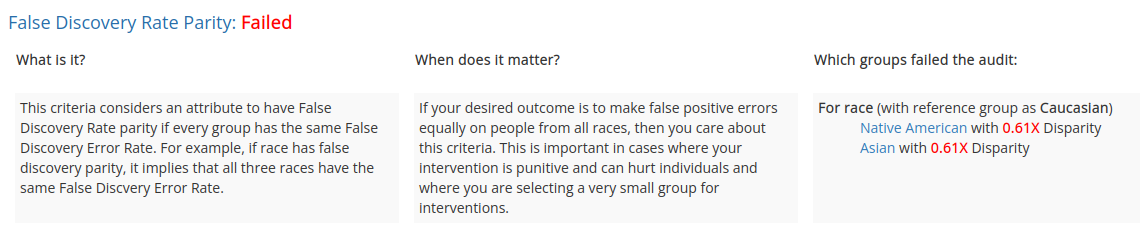
\includegraphics[width=16.7cm]{fairness_adult_output2.png}
	\caption{Resultado injusto para la paridad métrica FDR con $\tau=0.8$.}
    \label{fig:ejunfairaq2}
\end{figure}

Si cambiamos la regla $p$\% de un 80\% a, por ejemplo, un 60\%, el intervalo del umbral para $\tau=0.6$ sería $[0.6,1.67]$, obteniendo los siguientes resultados.\\

\begin{table}[h]
\centering
\resizebox{14.cm}{!} {
\begin{tabular}{ccccccc}
{\color[HTML]{3166FF} race}                                                              & \multicolumn{1}{l}{}                                                                  & \multicolumn{1}{l}{}                                                                    & \multicolumn{1}{l}{}                                                                  & \multicolumn{1}{l}{}                                                                  & \multicolumn{1}{l}{}                                                                  & \multicolumn{1}{l}{}                                                                  \\
{\color[HTML]{3166FF} }                                                                  & \multicolumn{1}{l}{}                                                                  & \multicolumn{1}{l}{}                                                                    & \multicolumn{1}{l}{}                                                                  & \multicolumn{1}{l}{}                                                                  & \multicolumn{1}{l}{}                                                                  & \multicolumn{1}{l}{}                                                                  \\ \hline
\multicolumn{1}{|c|}{\textbf{\begin{tabular}[c]{@{}c@{}}Attribute\\ Value\end{tabular}}} & \multicolumn{1}{c|}{\textbf{\begin{tabular}[c]{@{}c@{}}PPR\\ Disparity\end{tabular}}} & \multicolumn{1}{c|}{\textbf{\begin{tabular}[c]{@{}c@{}}PPREV\\ Disparity\end{tabular}}} & \multicolumn{1}{c|}{\textbf{\begin{tabular}[c]{@{}c@{}}FDR\\ Disparity\end{tabular}}} & \multicolumn{1}{c|}{\textbf{\begin{tabular}[c]{@{}c@{}}FPR\\ Disparity\end{tabular}}} & \multicolumn{1}{c|}{\textbf{\begin{tabular}[c]{@{}c@{}}FOR\\ Disparity\end{tabular}}} & \multicolumn{1}{c|}{\textbf{\begin{tabular}[c]{@{}c@{}}FNR\\ Disparity\end{tabular}}} \\ \hline
\multicolumn{1}{|c|}{\begin{tabular}[c]{@{}c@{}}African-\\ American\end{tabular}}        & \multicolumn{1}{c|}{{\color[HTML]{FE0000} 2.55}}                                      & \multicolumn{1}{c|}{{\color[HTML]{FE0000} 1.69}}                                        & \multicolumn{1}{c|}{{\color[HTML]{32CB00} 0.91}}                                      & \multicolumn{1}{c|}{{\color[HTML]{FE0000} 1.91}}                                      & \multicolumn{1}{c|}{{\color[HTML]{32CB00} 1.21}}                                      & \multicolumn{1}{c|}{{\color[HTML]{FE0000} 0.59}}                                      \\ \hline
\multicolumn{1}{|c|}{Asian}                                                              & \multicolumn{1}{c|}{{\color[HTML]{FE0000} 0.01}}                                      & \multicolumn{1}{c|}{{\color[HTML]{32CB00} 0.72}}                                        & \multicolumn{1}{c|}{{\color[HTML]{32CB00} 0.61}}                                      & \multicolumn{1}{c|}{{\color[HTML]{FE0000} 0.37}}                                      & \multicolumn{1}{c|}{{\color[HTML]{FE0000} 0.43}}                                      & \multicolumn{1}{c|}{{\color[HTML]{32CB00} 0.7}}                                       \\ \hline
\multicolumn{1}{|c|}{Caucasian}                                                          & \multicolumn{1}{c|}{{\color[HTML]{3166FF} 1.0}}                                       & \multicolumn{1}{c|}{{\color[HTML]{3166FF} 1.0}}                                         & \multicolumn{1}{c|}{{\color[HTML]{3166FF} 1.0}}                                       & \multicolumn{1}{c|}{{\color[HTML]{3166FF} 1.0}}                                       & \multicolumn{1}{c|}{{\color[HTML]{3166FF} 1.0}}                                       & \multicolumn{1}{c|}{{\color[HTML]{3166FF} 1.0}}                                       \\ \hline
\multicolumn{1}{|c|}{Hispanic}                                                           & \multicolumn{1}{c|}{{\color[HTML]{FE0000} 0.22}}                                      & \multicolumn{1}{c|}{{\color[HTML]{32CB00} 0.86}}                                        & \multicolumn{1}{c|}{{\color[HTML]{32CB00} 1.12}}                                      & \multicolumn{1}{c|}{{\color[HTML]{32CB00} 0.92}}                                      & \multicolumn{1}{c|}{{\color[HTML]{32CB00} 1.0}}                                       & \multicolumn{1}{c|}{{\color[HTML]{32CB00} 1.17}}                                      \\ \hline
\multicolumn{1}{|c|}{\begin{tabular}[c]{@{}c@{}}Native\\ American\end{tabular}}          & \multicolumn{1}{c|}{{\color[HTML]{FE0000} 0.01}}                                      & \multicolumn{1}{c|}{{\color[HTML]{FE0000} 1.92}}                                        & \multicolumn{1}{c|}{{\color[HTML]{32CB00} 0.61}}                                      & \multicolumn{1}{c|}{{\color[HTML]{32CB00} 1.6}}                                       & \multicolumn{1}{c|}{{\color[HTML]{FE0000} 0.58}}                                      & \multicolumn{1}{c|}{{\color[HTML]{FE0000} 0.21}}                                      \\ \hline
\multicolumn{1}{|c|}{Other}                                                              & \multicolumn{1}{c|}{{\color[HTML]{FE0000} 0.09}}                                      & \multicolumn{1}{c|}{{\color[HTML]{32CB00} 0.6}}                                         & \multicolumn{1}{c|}{{\color[HTML]{32CB00} 1.12}}                                      & \multicolumn{1}{c|}{{\color[HTML]{32CB00} 0.63}}                                      & \multicolumn{1}{c|}{{\color[HTML]{32CB00} 1.05}}                                      & \multicolumn{1}{c|}{{\color[HTML]{32CB00} 1.42}}                                      \\ \hline
\end{tabular}
}
	\caption{Tabla con las métricas de disparidad para el atributo \textit{race} con umbral del 60\%.}
    \label{fig:ejaq22}
\end{table}

En la Tabla \ref{fig:ejaq22} podemos observar que la paridad de la tasa de falso descubrimiento (FDR) tiene todos los valores de su columna en verde. Aequitas indicará entonces que, basándonos en el umbral establecido ($\tau=0.6$), todos los grupos cumplen la definición de la métrica y por tanto considera justo el concepto de FDR Parity.

\subsection*{Estudio de la equidad}

Finalmente utilizaremos la clase \textit{Fairness()} para hacer un estudio más exhaustivo sobre los criterios de paridad estudiados en la Tabla \ref{fig:ejaq2}.

La Figura \ref{fig:compasdgroup} muestra los resultados detallados de algunas de las métricas de grupo más populares: las barras verdes representan los grupos para los que el modelo no presenta un sesgo dentro de esa métrica, mientras que las barras rojas indican un sesgo desfavorable en comparación con el grupo de referencia. Seguimos utilizando el umbral de equidad $\tau = 0.8$. Los resultados muestran que para cada métrica existe al menos un grupo con algún tipo de sesgo respecto al grupo de referencia. \textit{COMPAS} considera mayoritariamente como de alto riesgo a los menores de 25 años, a los hombres y a los afroamericanos. Según las métricas PPR, que muestran las entidades con \textit{score}=1; vemos que, en comparación con el tamaño de cada grupo, los más jóvenes, los nativos-americanos y los afroamericanos son seleccionados de forma desproporcionada.

Para visualizar las disparidades entre los distintos grupos, la herramienta también produce resultados para las métricas de disparidad. A continuación tenemos que determinar qué medida de sesgo es relevante para nuestro entorno. Dado que en el marco del \textit{COMPAS}, las predicciones se utilizan para tomar decisiones de liberación previa al juicio, las intervenciones serán punitivas (proporcionar esta intervención a los individuos que son falsos positivos les perjudicará), así que deberemos tener en cuenta las tasas de falsos descubrimientos (FDR) y las tasas de falsos positivos (FPR).

\clearpage

\begin{figure}[h]
	\hspace{-2.5cm}
	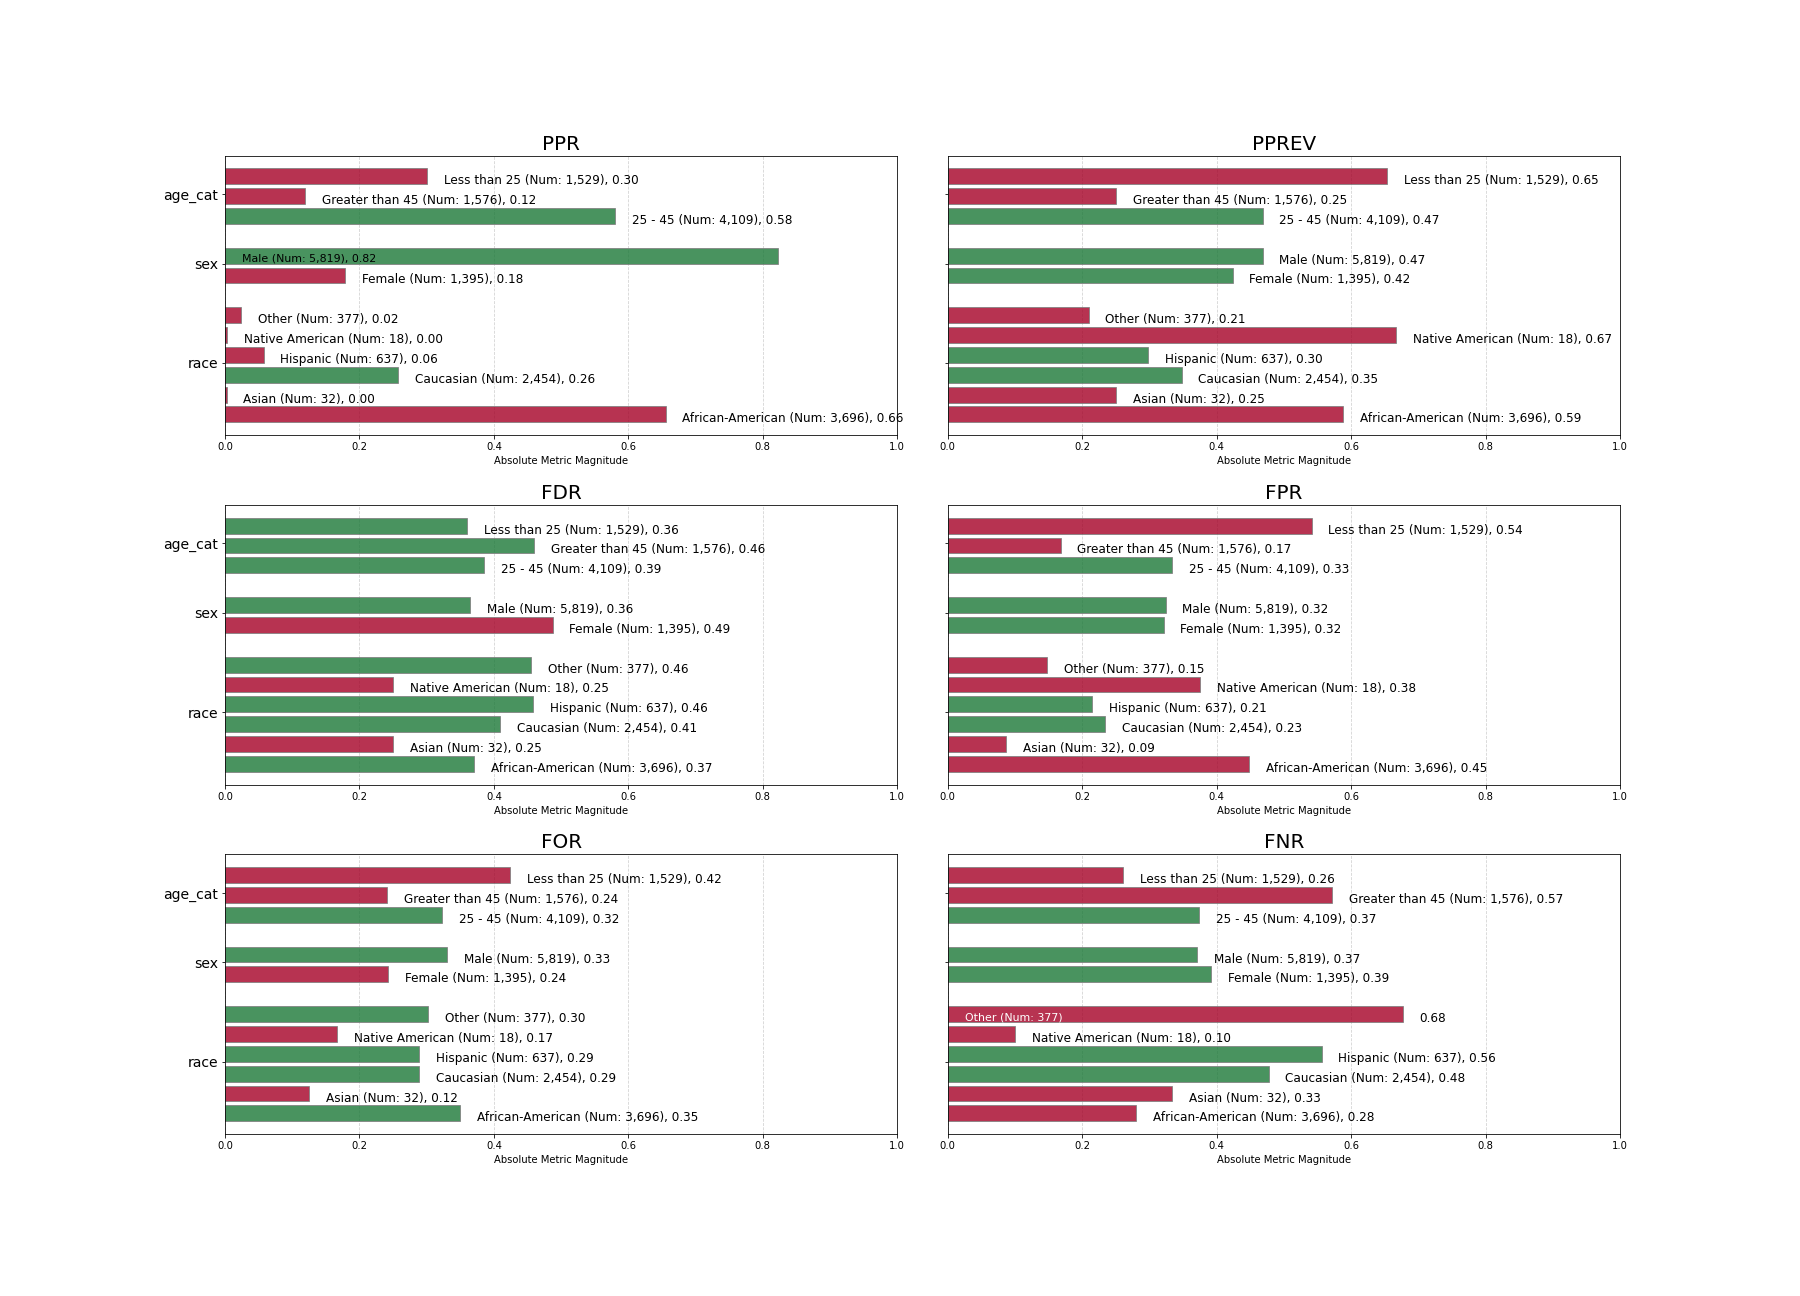
\includegraphics[width=21.3cm]{disparity_group.png}
	\caption{Resultado de las métricas de grupo para COMPAS con $\tau=0.8$.}
    \label{fig:compasdgroup}
\end{figure}

Observando la Figura \ref{fig:compasdisparity} podemos ver que el conjunto de datos \textit{COMPAS} es justo para la métrica FDR para la raza, pero la FPR para los afroamericanos es casi el doble que para los caucásicos, por lo que existe un problema evidente de sesgo. También existen problemas de sesgo para los atributos de sexo y edad. En cuanto al sexo, los resultados del FPR son justos, pero el FDR para las mujeres es 1.34 veces mayor que el de los hombres. Por otro lado, si consideramos la distribución de errores falsos positivos teniendo en cuenta la edad, observamos lo contrario: el modelo es justo para el FDR, pero el FPR para los menores de 25 años es 1.62 veces mayor que el de 25-45.

\clearpage

\begin{figure}[h]
	\hspace{-2.5cm}
	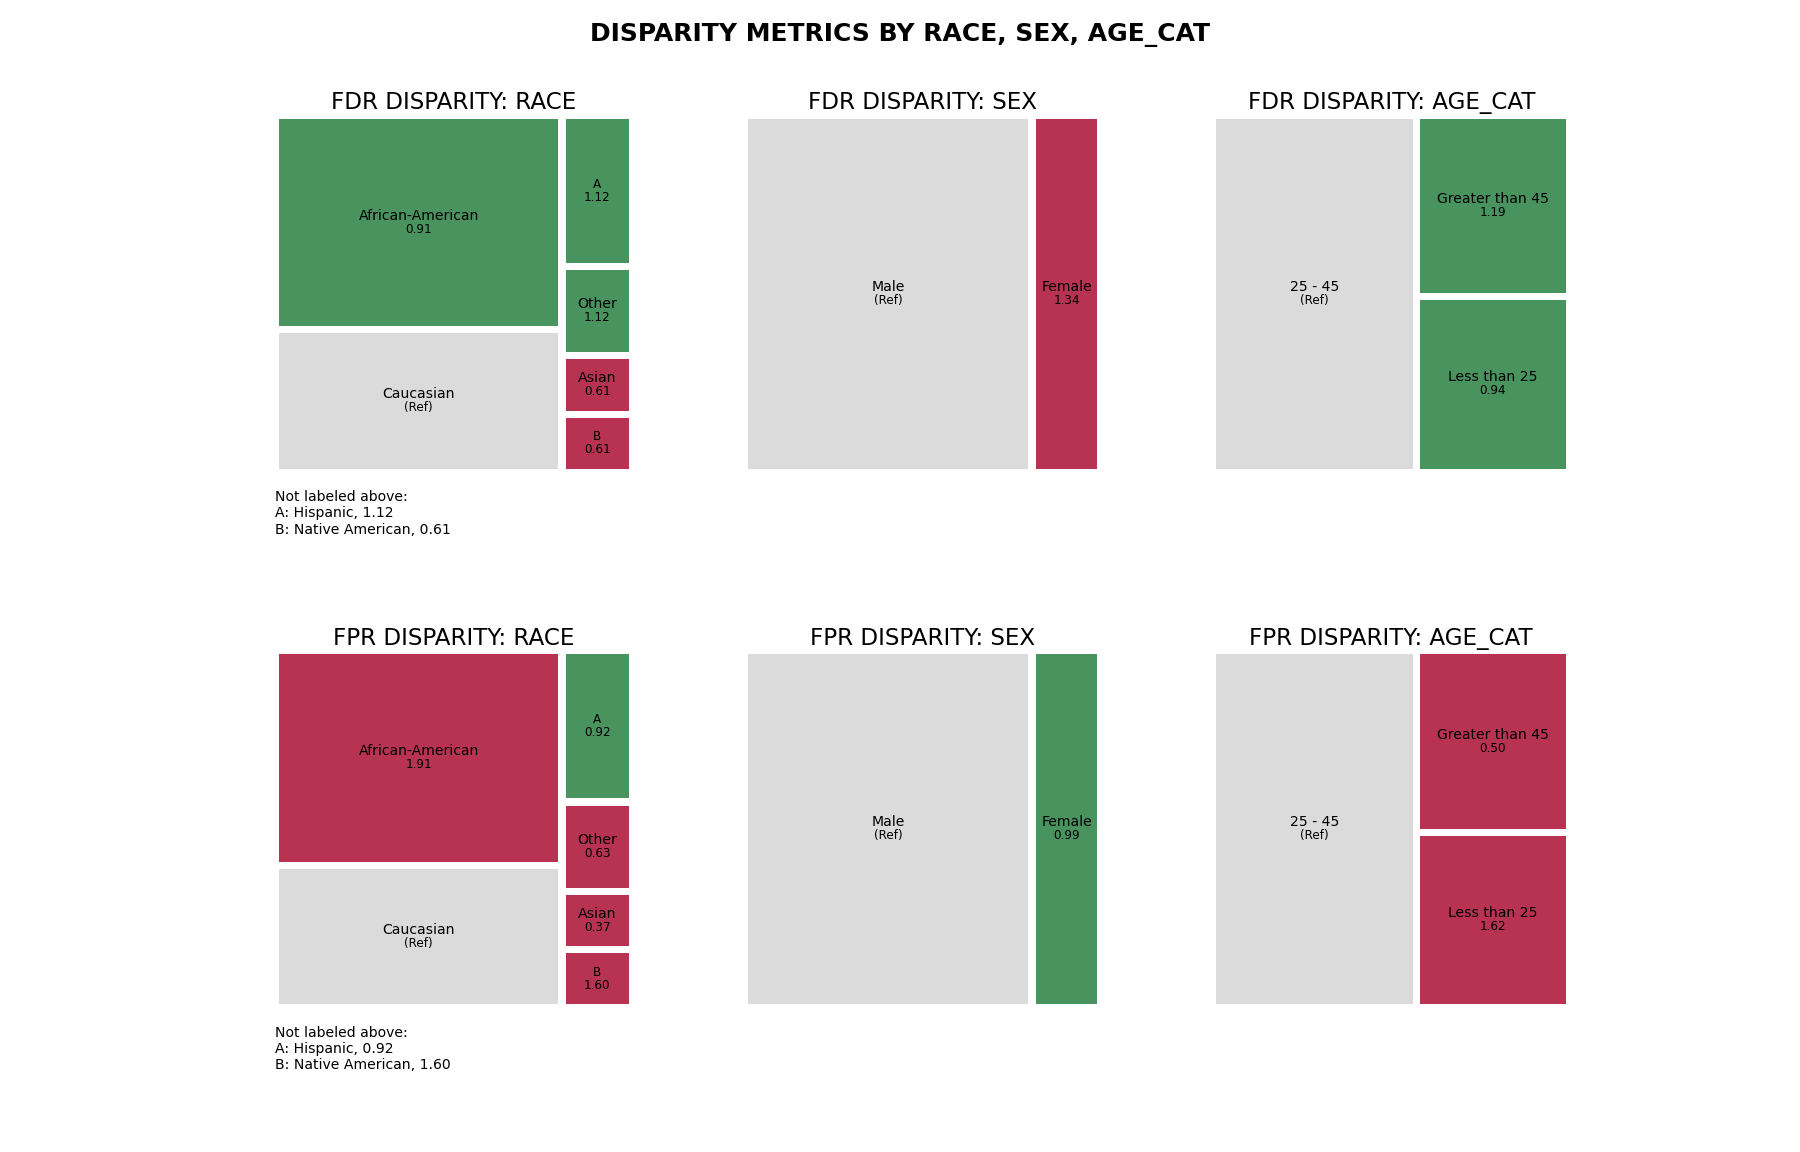
\includegraphics[width=21.3cm]{disparity.png}
	\caption{Resultado de las métricas de disparidad para \textit{COMPAS} con $\tau=0.8$.}
    \label{fig:compasdisparity}
\end{figure}

\subsection{Ejemplo: Predicción de notas en la facultad de derecho} \label{ap:facultadderecho}

Analizaremos el ejemplo sobre el conjunto de datos \textit{law\_data} que presentamos en el Apartado \ref{subsec:desproblem} de nuestra fase experimental. Para tratar la puntuación de riesgo con Aequitas, convertiremos el \textit{score} original (FYA), que toma valores en el intervalo $(-2.5,2.5)$, a uno binario: donde 0 indicará una nota baja en el primer año de carrera y 1 una nota alta.

Además eliminaremos cualquier atributo que pudiera entorpecer al estudio de los datos en Aequitas, quedándonos  únicamente con las columnas que contienen los valores para los dos atributos protegidos del problema (sexo y raza), la columna con los nuevos valores de \textit{score} y la columna de \textit{label\_value}, cuyo valor binario indica la decisión real que fue tomada en el problema.

\clearpage

\begin{table}[h]
\centering
\resizebox{7.5cm}{!} {
\begin{tabular}{|c|c|c|c|}
\hline
\textbf{score} & \textbf{label\_value} & \textbf{race}    & \textbf{sex} \\ \hline
1            & 1                     & White & Female       \\ \hline
1              & 1                     & Asian         & Male      \\ \hline
0              & 1                     & Black       & Male              \\ \hline
\end{tabular}
}
\caption{Ejemplo del \textit{dataset law\_data} aportado a Aequitas.}
\label{tab:ejlawaeq}
\end{table}

En la Tabla \ref{tab:distribuciongrupo}, realizamos un estudio previo de la fracción sobre el total de individuos por raza de cada una de las categorías existentes.\\

\begin{table}[h]
\centering
\resizebox{9.5cm}{!} {
\begin{tabular}{|c|c|c|c|}
\hline
\textbf{\begin{tabular}[c]{@{}c@{}}Attribute\\ Value\end{tabular}} & \textbf{\begin{tabular}[c]{@{}c@{}}Group Size\\ Ratio\end{tabular}} & \textbf{\begin{tabular}[c]{@{}c@{}}Attribute\\ Value\end{tabular}} & \textbf{\begin{tabular}[c]{@{}c@{}}Group Size\\ Ratio\end{tabular}} \\ \hline
Amerindian                                                         & 0                                                                   & Mexican                                                            & 0.02                                                                \\ \hline
Asian                                                              & 0.04                                                                & Other                                                              & 0.01                                                                \\ \hline
Black                                                              & 0.06                                                                & Puertorican                                                        & 0.01                                                                \\ \hline
Hispanic                                                           & 0.02                                                                & White                                                              & 0.84                                                                \\ \hline
\end{tabular}
}
\caption{Distribución de los individuos por \textit{raza}.}
\label{tab:distribuciongrupo}
\end{table}

Como queremos realizar un análisis lo más general posible, agruparemos los individuos de razas con una representación demasiado pequeña en otra categoría ya existente, en la que puedan figurar. Para ello, añadiremos a la categoría raza hispánica a los individuos de raza mexicana y puertorriqueña, y a la categoría otras a los sujetos de raza amerindia.

\subsection*{Análisis de los datos}

En los gráficos siguientes podemos notar una gran diferencia en la distribución de las puntuaciones por raza (Figura \ref{fig:barrasracelaw}), con una mayoría de personas de raza blanca pronosticadas con notas altas en el primer año (\textit{score}=1), y una mayoría de población negra e hispánica pronosticada con puntuación baja (\textit{score}=0). En cuanto al atributo sexo (Figura \ref{fig:barrasage}), parece que, en principio, no es determinante a la hora de puntuar, aunque existen más individuos de sexo masculino que femeninos puntuados como aptos.

Mostramos mediante varios gráficos cómo se distribuyen las etiquetas reales según los atributos protegidos. Las etiquetas reales contienen la información real sobre si el individuo obtuvo una calificación alta en su primer año (\textit{label\_value}=1) o no (\textit{label\_value}=0). Con esta información podremos comprobar directamente la precisión de las predicciones.

\clearpage

\begin{figure}[h]
    \minipage{0.53\textwidth}
      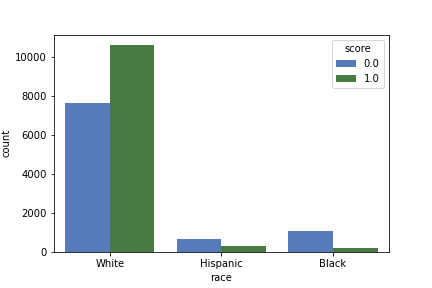
\includegraphics[width=\linewidth]{images/score_race_law.png}
    \endminipage\hfill
    \minipage{0.53\textwidth}%
      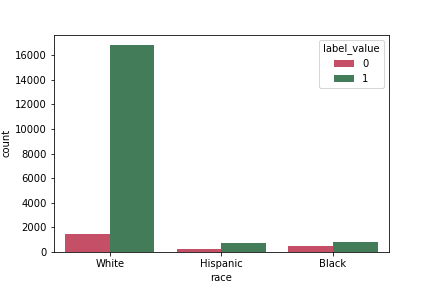
\includegraphics[width=\linewidth]{images/label_race_law.png}
    \endminipage
     \caption{Gráfico de barras de la puntuación y etiqueta real para el atributo \textit{race}.}
     \label{fig:barrasracelaw}
\end{figure}

\begin{figure}[h]
    \minipage{0.53\textwidth}
      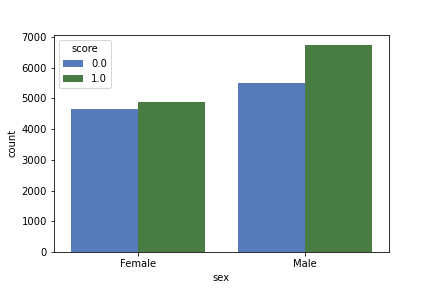
\includegraphics[width=\linewidth]{images/score_sex_law.png}
    \endminipage\hfill
    \minipage{0.53\textwidth}%
      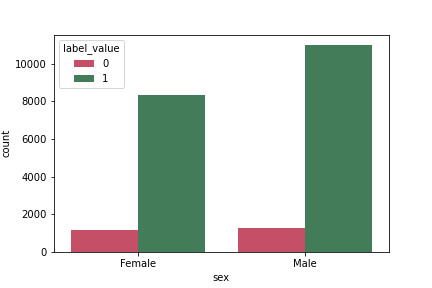
\includegraphics[width=\linewidth]{images/label_sex_law.png}
    \endminipage
     \caption{Gráfico de barras de la puntuación y etiqueta real para el atributo \textit{sex}.}
     \label{fig:barrassexlaw}
\end{figure}

En la Figura \ref{fig:barrasracelaw} podemos observar que donde se detecta una mayor diferencia entre las gráficas de puntuación y etiquetas reales es en el grupo de los individuos de raza negra e hispánica. Además, la distribución de etiquetas reales para el atributo sexo de la Figura \ref{fig:barrassexlaw} deja ver que hay muchos individuos que se puntúan con \textit{score}=0, y que finalmente acaban obteniendo buenas notas. Para realizar un estudio de los datos utilizaremos la herramienta de Aequitas, analizando los posibles patrones de sesgo que pudiesen existir entre los diferentes grupos de la población del conjunto de datos \textit{law\_data}.

\subsection*{Métricas de grupo}

Usando la clase \textit{Group()} calcularemos los valores de las métricas de grupo para los atributos de raza y sexo. Observamos en la Tabla \ref{fig:ejaq1law} que la mayoría de los individuos son de raza blanca y el resto de categorías está medianamente equilibrada en cuanto a grupos de población. Por otro lado, la Tabla \ref{fig:ejaq2law} muestra que la distribución del atributo sexo contiene una proporción mínimamente mayor de hombres que de mujeres.\\

\begin{table}[h]
\centering
\resizebox{12.6cm}{!} {
\begin{tabular}{cccccccc}
{\color[HTML]{3166FF} race}                                                              & \multicolumn{1}{l}{}                                                                     & \multicolumn{1}{l}{}                             & \multicolumn{1}{l}{}                             & \multicolumn{1}{l}{}                             & \multicolumn{1}{l}{}                             & \multicolumn{1}{l}{}                             & \multicolumn{1}{l}{}                             \\
{\color[HTML]{3166FF} }                                                                  & \multicolumn{1}{l}{}                                                                     & \multicolumn{1}{l}{}                             & \multicolumn{1}{l}{}                             & \multicolumn{1}{l}{}                             & \multicolumn{1}{l}{}                             & \multicolumn{1}{l}{}                             & \multicolumn{1}{l}{}                             \\ \hline
\multicolumn{1}{|c|}{\textbf{\begin{tabular}[c]{@{}c@{}}Attribute\\ Value\end{tabular}}} & \multicolumn{1}{c|}{\textbf{\begin{tabular}[c]{@{}c@{}}Group Size\\ Ratio\end{tabular}}} & \multicolumn{1}{c|}{\textbf{PPR}}                & \multicolumn{1}{c|}{\textbf{PPREV}}              & \multicolumn{1}{c|}{\textbf{FDR}}                & \multicolumn{1}{c|}{\textbf{FPR}}                & \multicolumn{1}{c|}{\textbf{FOR}}                & \multicolumn{1}{c|}{\textbf{FNR}}                \\ \hline
\multicolumn{1}{|c|}{\begin{tabular}[c]{@{}c@{}}Asian\end{tabular}}        & \multicolumn{1}{c|}{0.04}                                                                & \multicolumn{1}{c|}{{0.02}} & \multicolumn{1}{c|}{{0.34}} & \multicolumn{1}{c|}{{0.06}} & \multicolumn{1}{c|}{{0.1}} & \multicolumn{1}{c|}{{0.75}} & \multicolumn{1}{c|}{{0.61}} \\ \hline
\multicolumn{1}{|c|}{Black}                                                              & \multicolumn{1}{c|}{0.06}                                                                   & \multicolumn{1}{c|}{{0.02}}  & \multicolumn{1}{c|}{{ 0.18}} & \multicolumn{1}{c|}{{ 0.15}} & \multicolumn{1}{c|}{{0.07}} & \multicolumn{1}{c|}{{ 0.57}} & \multicolumn{1}{c|}{{0.76}} \\ \hline
\multicolumn{1}{|c|}{Hispanic}                                                          & \multicolumn{1}{c|}{0.05}                                                                & \multicolumn{1}{c|}{0.03}                        & \multicolumn{1}{c|}{0.32}                        & \multicolumn{1}{c|}{0.08}                        & \multicolumn{1}{c|}{0.1}                        & \multicolumn{1}{c|}{0.67}                        & \multicolumn{1}{c|}{0.61}                        \\ \hline
\multicolumn{1}{|c|}{Other}                                                           & \multicolumn{1}{c|}{0.02}                                                                & \multicolumn{1}{c|}{{0.01}} & \multicolumn{1}{c|}{{ 0.41}}  & \multicolumn{1}{c|}{{ 0.02}} & \multicolumn{1}{c|}{{ 0.05}} & \multicolumn{1}{c|}{{ 0.67}} & \multicolumn{1}{c|}{{ 0.5}} \\ \hline
\multicolumn{1}{|c|}{\begin{tabular}[c]{@{}c@{}}White\end{tabular}}          & \multicolumn{1}{c|}{0.84}                                                                   & \multicolumn{1}{c|}{{ 0.91}}  & \multicolumn{1}{c|}{{ 0.58}} & \multicolumn{1}{c|}{{ 0.03}} & \multicolumn{1}{c|}{{ 0.2}} & \multicolumn{1}{c|}{{ 0.85}} & \multicolumn{1}{c|}{{ 0.39}}  \\ \hline
\end{tabular}
}
	\caption{Tabla con las principales métricas de grupo para el atributo \textit{race}.}
    \label{fig:ejaq1law}
\end{table}

\begin{table}[h]
\centering
\resizebox{12.cm}{!} {
\begin{tabular}{cccccccc}
{\color[HTML]{3166FF} sex}                                                              & \multicolumn{1}{l}{}                                                                     & \multicolumn{1}{l}{}                             & \multicolumn{1}{l}{}                             & \multicolumn{1}{l}{}                             & \multicolumn{1}{l}{}                             & \multicolumn{1}{l}{}                             & \multicolumn{1}{l}{}                             \\
{\color[HTML]{3166FF} }                                                                  & \multicolumn{1}{l}{}                                                                     & \multicolumn{1}{l}{}                             & \multicolumn{1}{l}{}                             & \multicolumn{1}{l}{}                             & \multicolumn{1}{l}{}                             & \multicolumn{1}{l}{}                             & \multicolumn{1}{l}{}                             \\ \hline
\multicolumn{1}{|c|}{\textbf{\begin{tabular}[c]{@{}c@{}}Attribute\\ Value\end{tabular}}} & \multicolumn{1}{c|}{\textbf{\begin{tabular}[c]{@{}c@{}}Group Size\\ Ratio\end{tabular}}} & \multicolumn{1}{c|}{\textbf{PPR}}                & \multicolumn{1}{c|}{\textbf{PPREV}}              & \multicolumn{1}{c|}{\textbf{FDR}}                & \multicolumn{1}{c|}{\textbf{FPR}}                & \multicolumn{1}{c|}{\textbf{FOR}}                & \multicolumn{1}{c|}{\textbf{FNR}}                \\ \hline
\multicolumn{1}{|c|}{\begin{tabular}[c]{@{}c@{}}Female\end{tabular}}        & \multicolumn{1}{c|}{0.44}                                                                & \multicolumn{1}{c|}{{0.42}} & \multicolumn{1}{c|}{{0.51}} & \multicolumn{1}{c|}{{0.03}} & \multicolumn{1}{c|}{{0.14}} & \multicolumn{1}{c|}{{0.78}} & \multicolumn{1}{c|}{{0.44}} \\ \hline
\multicolumn{1}{|c|}{Male}                                                              & \multicolumn{1}{c|}{0.56}                                                                   & \multicolumn{1}{c|}{{0.58}}  & \multicolumn{1}{c|}{{ 0.55}} & \multicolumn{1}{c|}{{ 0.03}} & \multicolumn{1}{c|}{{0.16}} & \multicolumn{1}{c|}{{ 0.81}} & \multicolumn{1}{c|}{{0.41}} \\ \hline
\end{tabular}
}
	\caption{Tabla con las principales métricas de grupo para el atributo \textit{sex}.}
    \label{fig:ejaq2law}
\end{table}

\subsection*{Métricas de disparidad}

Tomaremos como atributos de referencia la raza \textit{White} y el sexo \textit{Male}, por ser tanto los mayoritarios, como los valores que históricamente sufren menos impacto dispar.

A continuación usaremos la clase \textit{Bias()} para medir la disparidad entre cada grupo objetivo y los grupos de referencia seleccionados. 

Veamos un ejemplo de cómo realiza el cálculo Aequitas en este caso concreto. Mediremos la disparidad para la tasa de falsa omisión (FOR) sobre el grupo de raza \textit{Black} y el grupo de sexo \textit{Female}:
$$\text{FOR}_{\text{G(Black)}}=\ddfrac{\text{FOR}_{\text{Black}}}{\text{FOR}_{\text{White}}}=\ddfrac{0.57}{0.85}=0.67.$$
$$\text{FOR}_{\text{G(Female)}}=\ddfrac{\text{FOR}_{\text{Female}}}{\text{FOR}_{\text{Male}}}=\ddfrac{0.78}{0.81}=0.97.$$

Completando la tabla con las métricas de disparidad para todas las métricas de grupo obtendremos los siguientes resultados:

\begin{table}[h]
\centering
\resizebox{14.cm}{!} {
\begin{tabular}{ccccccc}
{\color[HTML]{3166FF} race}                                                              & \multicolumn{1}{l}{}                                                                  & \multicolumn{1}{l}{}                                                                    & \multicolumn{1}{l}{}                                                                  & \multicolumn{1}{l}{}                                                                  & \multicolumn{1}{l}{}                                                                  & \multicolumn{1}{l}{}                                                                  \\
\multicolumn{1}{l}{}                                                                     & \multicolumn{1}{l}{}                                                                  & \multicolumn{1}{l}{}                                                                    & \multicolumn{1}{l}{}                                                                  & \multicolumn{1}{l}{}                                                                  & \multicolumn{1}{l}{}                                                                  & \multicolumn{1}{l}{}                                                                  \\ \hline
\multicolumn{1}{|c|}{\textbf{\begin{tabular}[c]{@{}c@{}}Attribute\\ Value\end{tabular}}} & \multicolumn{1}{c|}{\textbf{\begin{tabular}[c]{@{}c@{}}PPR\\ Disparity\end{tabular}}} & \multicolumn{1}{c|}{\textbf{\begin{tabular}[c]{@{}c@{}}PPREV\\ Disparity\end{tabular}}} & \multicolumn{1}{c|}{\textbf{\begin{tabular}[c]{@{}c@{}}FDR\\ Disparity\end{tabular}}} & \multicolumn{1}{c|}{\textbf{\begin{tabular}[c]{@{}c@{}}FPR\\ Disparity\end{tabular}}} & \multicolumn{1}{c|}{\textbf{\begin{tabular}[c]{@{}c@{}}FOR\\ Disparity\end{tabular}}} & \multicolumn{1}{c|}{\textbf{\begin{tabular}[c]{@{}c@{}}FNR\\ Disparity\end{tabular}}} \\ \hline
\multicolumn{1}{|c|}{Asian}                                                              & \multicolumn{1}{c|}{{\color[HTML]{FE0000} 0.03}}                                      & \multicolumn{1}{c|}{{\color[HTML]{FE0000} 0.58}}                                        & \multicolumn{1}{c|}{{\color[HTML]{FE0000} 2.07}}                                      & \multicolumn{1}{c|}{{\color[HTML]{FE0000} 0.52}}                                      & \multicolumn{1}{c|}{{\color[HTML]{32CB00} 0.88}}                                      & \multicolumn{1}{c|}{{\color[HTML]{FE0000} 1.58}}                                      \\ \hline
\multicolumn{1}{|c|}{Black}                                                              & \multicolumn{1}{c|}{{\color[HTML]{FE0000} 0.02}}                                      & \multicolumn{1}{c|}{{\color[HTML]{FE0000} 0.3}}                                         & \multicolumn{1}{c|}{{\color[HTML]{FE0000} 5.59}}                                      & \multicolumn{1}{c|}{{\color[HTML]{FE0000} 0.35}}                                      & \multicolumn{1}{c|}{{\color[HTML]{FE0000} 0.67}}                                      & \multicolumn{1}{c|}{{\color[HTML]{FE0000} 1.97}}                                      \\ \hline
\multicolumn{1}{|c|}{Hispanic}                                                           & \multicolumn{1}{c|}{{\color[HTML]{FE0000} 0.03}}                                      & \multicolumn{1}{c|}{{\color[HTML]{FE0000} 0.55}}                                        & \multicolumn{1}{c|}{{\color[HTML]{FE0000} 2.84}}                                      & \multicolumn{1}{c|}{{\color[HTML]{FE0000} 0.49}}                                      & \multicolumn{1}{c|}{{\color[HTML]{FE0000} 0.79}}                                      & \multicolumn{1}{c|}{{\color[HTML]{FE0000} 1.58}}                                      \\ \hline
\multicolumn{1}{|c|}{Other}                                                              & \multicolumn{1}{c|}{{\color[HTML]{FE0000} 0.02}}                                      & \multicolumn{1}{c|}{{\color[HTML]{FE0000} 0.71}}                                        & \multicolumn{1}{c|}{{\color[HTML]{32CB00} 0.92}}                                      & \multicolumn{1}{c|}{{\color[HTML]{FE0000} 0.26}}                                      & \multicolumn{1}{c|}{{\color[HTML]{FE0000} 0.8}}                                       & \multicolumn{1}{c|}{{\color[HTML]{FE0000} 1.29}}                                      \\ \hline
\multicolumn{1}{|c|}{White}                                                              & \multicolumn{1}{c|}{{\color[HTML]{3166FF} 1.0}}                                       & \multicolumn{1}{c|}{{\color[HTML]{3166FF} 1.0}}                                         & \multicolumn{1}{c|}{{\color[HTML]{3166FF} 1.0}}                                       & \multicolumn{1}{c|}{{\color[HTML]{3166FF} 1.0}}                                       & \multicolumn{1}{c|}{{\color[HTML]{3166FF} 1.0}}                                       & \multicolumn{1}{c|}{{\color[HTML]{3166FF} 1.0}}                                       \\ \hline
\end{tabular}
}
	\caption{Tabla con las métricas de disparidad para el atributo \textit{race} con umbral del 80\%.}
    \label{fig:ejaqracelaw}
\end{table}

\begin{table}[h]
\centering
\resizebox{14.cm}{!} {
\begin{tabular}{ccccccc}
{\color[HTML]{3166FF} sex}                                                               & \multicolumn{1}{l}{}                                                                  & \multicolumn{1}{l}{}                                                                    & \multicolumn{1}{l}{}                                                                  & \multicolumn{1}{l}{}                                                                  & \multicolumn{1}{l}{}                                                                  & \multicolumn{1}{l}{}                                                                  \\
\multicolumn{1}{l}{}                                                                     & \multicolumn{1}{l}{}                                                                  & \multicolumn{1}{l}{}                                                                    & \multicolumn{1}{l}{}                                                                  & \multicolumn{1}{l}{}                                                                  & \multicolumn{1}{l}{}                                                                  & \multicolumn{1}{l}{}                                                                  \\ \hline
\multicolumn{1}{|c|}{\textbf{\begin{tabular}[c]{@{}c@{}}Attribute\\ Value\end{tabular}}} & \multicolumn{1}{c|}{\textbf{\begin{tabular}[c]{@{}c@{}}PPR\\ Disparity\end{tabular}}} & \multicolumn{1}{c|}{\textbf{\begin{tabular}[c]{@{}c@{}}PPREV\\ Disparity\end{tabular}}} & \multicolumn{1}{c|}{\textbf{\begin{tabular}[c]{@{}c@{}}FDR\\ Disparity\end{tabular}}} & \multicolumn{1}{c|}{\textbf{\begin{tabular}[c]{@{}c@{}}FPR\\ Disparity\end{tabular}}} & \multicolumn{1}{c|}{\textbf{\begin{tabular}[c]{@{}c@{}}FOR\\ Disparity\end{tabular}}} & \multicolumn{1}{c|}{\textbf{\begin{tabular}[c]{@{}c@{}}FNR\\ Disparity\end{tabular}}} \\ \hline
\multicolumn{1}{|c|}{Female}                                                             & \multicolumn{1}{c|}{{\color[HTML]{FE0000} 0.72}}                                      & \multicolumn{1}{c|}{{\color[HTML]{32CB00} 0.93}}                                        & \multicolumn{1}{c|}{{\color[HTML]{32CB00} 1.16}}                                      & \multicolumn{1}{c|}{{\color[HTML]{32CB00} 0.89}}                                      & \multicolumn{1}{c|}{{\color[HTML]{32CB00} 0.97}}                                      & \multicolumn{1}{c|}{{\color[HTML]{32CB00} 1.08}}                                      \\ \hline
\multicolumn{1}{|c|}{Male}                                                               & \multicolumn{1}{c|}{{\color[HTML]{3166FF} 1.0}}                                       & \multicolumn{1}{c|}{{\color[HTML]{3166FF} 1.0}}                                         & \multicolumn{1}{c|}{{\color[HTML]{3166FF} 1.0}}                                       & \multicolumn{1}{c|}{{\color[HTML]{3166FF} 1.0}}                                       & \multicolumn{1}{c|}{{\color[HTML]{3166FF} 1.0}}                                       & \multicolumn{1}{c|}{{\color[HTML]{3166FF} 1.0}}                                       \\ \hline
\end{tabular}
}
	\caption{Tabla con las métricas de disparidad para el atributo \textit{sex} con umbral del 80\%.}
    \label{fig:ejaqsexlaw}
\end{table}

\subsection*{Medidas de equidad}

Para cumplir con la regla del 80\% tomamos $\tau=0.8$, por lo que cualquier métrica de disparidad se considerará justa si está contenida en el intervalo $[0.8,1.25]$.

En las Tablas \ref{fig:ejaqracelaw} y \ref{fig:ejaqsexlaw} destacamos en verde los valores contenidos en el intervalo, y en rojo los que se encuentran fuera del mismo. Si para todos los atributos existe una métrica de disparidad que contiene todos sus valores en color verde, el modelo se evaluará como justo. De lo contrario, lo considerará injusto. Podemos ver que para este conjunto de datos, y el umbral $\tau=0.8$, no se cumple ninguna medida de equidad.\\

\begin{table}[h]
\centering
\resizebox{17.cm}{!} {
\begin{tabular}{ll}
\textbf{Resumen de los resultados}                                                                                                                              &                              \\ \hline
Equal Parity - Todos los grupos protegidos tienen igual representación en el conjunto seleccionado.                                                     & {\color[HTML]{FE0000} Fallo} \\
Proportional Parity - Todos los grupos protegidos son seleccionados de forma proporcional a su porcentaje de la población                               & {\color[HTML]{FE0000} Fallo} \\
FPR Parity - Todos los grupos protegidos tienen la misma tasa de falsos positivos que el grupo de referencia.                                           & {\color[HTML]{FE0000} Fallo} \\
FDR Parity - Todos los grupos protegidos tienen igual proporción de falsos positivos entre el conjunto seleccionado (comparado con el de referencia)    & {\color[HTML]{FE0000} Fallo} \\
FNR Parity - Todos los grupos protegidos tienen la misma tasa de falsos negativos que el grupo de referencia.                                           & {\color[HTML]{FE0000} Fallo} \\
FOR Parity - Todos los grupos protegidos tienen igual proporción de falsos negativos entre el conjunto no seleccionado (comparado con el de referencia) & {\color[HTML]{FE0000} Fallo}
\end{tabular}
}
	\caption{Tabla de medidas de equidad con $\tau=0.8$.}
    \label{fig:medequmbral2}
\end{table}

\subsection*{Estudio de la equidad}

Finalmente utilizaremos la clase \textit{Fairness()} para hacer un estudio más exhaustivo sobre los criterios de paridad estudiados en las Tablas \ref{fig:ejaqracelaw} y \ref{fig:ejaqsexlaw}.

La Figura \ref{fig:lawdgroup} muestra los resultados detallados de algunas de las métricas de grupo más populares. Los resultados muestran que para cada métrica existe al menos un grupo con algún tipo de sesgo respecto al grupo de referencia. En el ámbito del problema, dado que las predicciones se utilizan para tomar decisiones de asistenciales (proporcionar esta asistencia a los individuos que son falsos positivos no les perjudicará), así que deberemos tener en cuenta las tasas de falsas omisiones (FOR) y las tasas de falsos negativos (FNR).\\

\begin{figure}[h]
	\hspace{-2.5cm}
	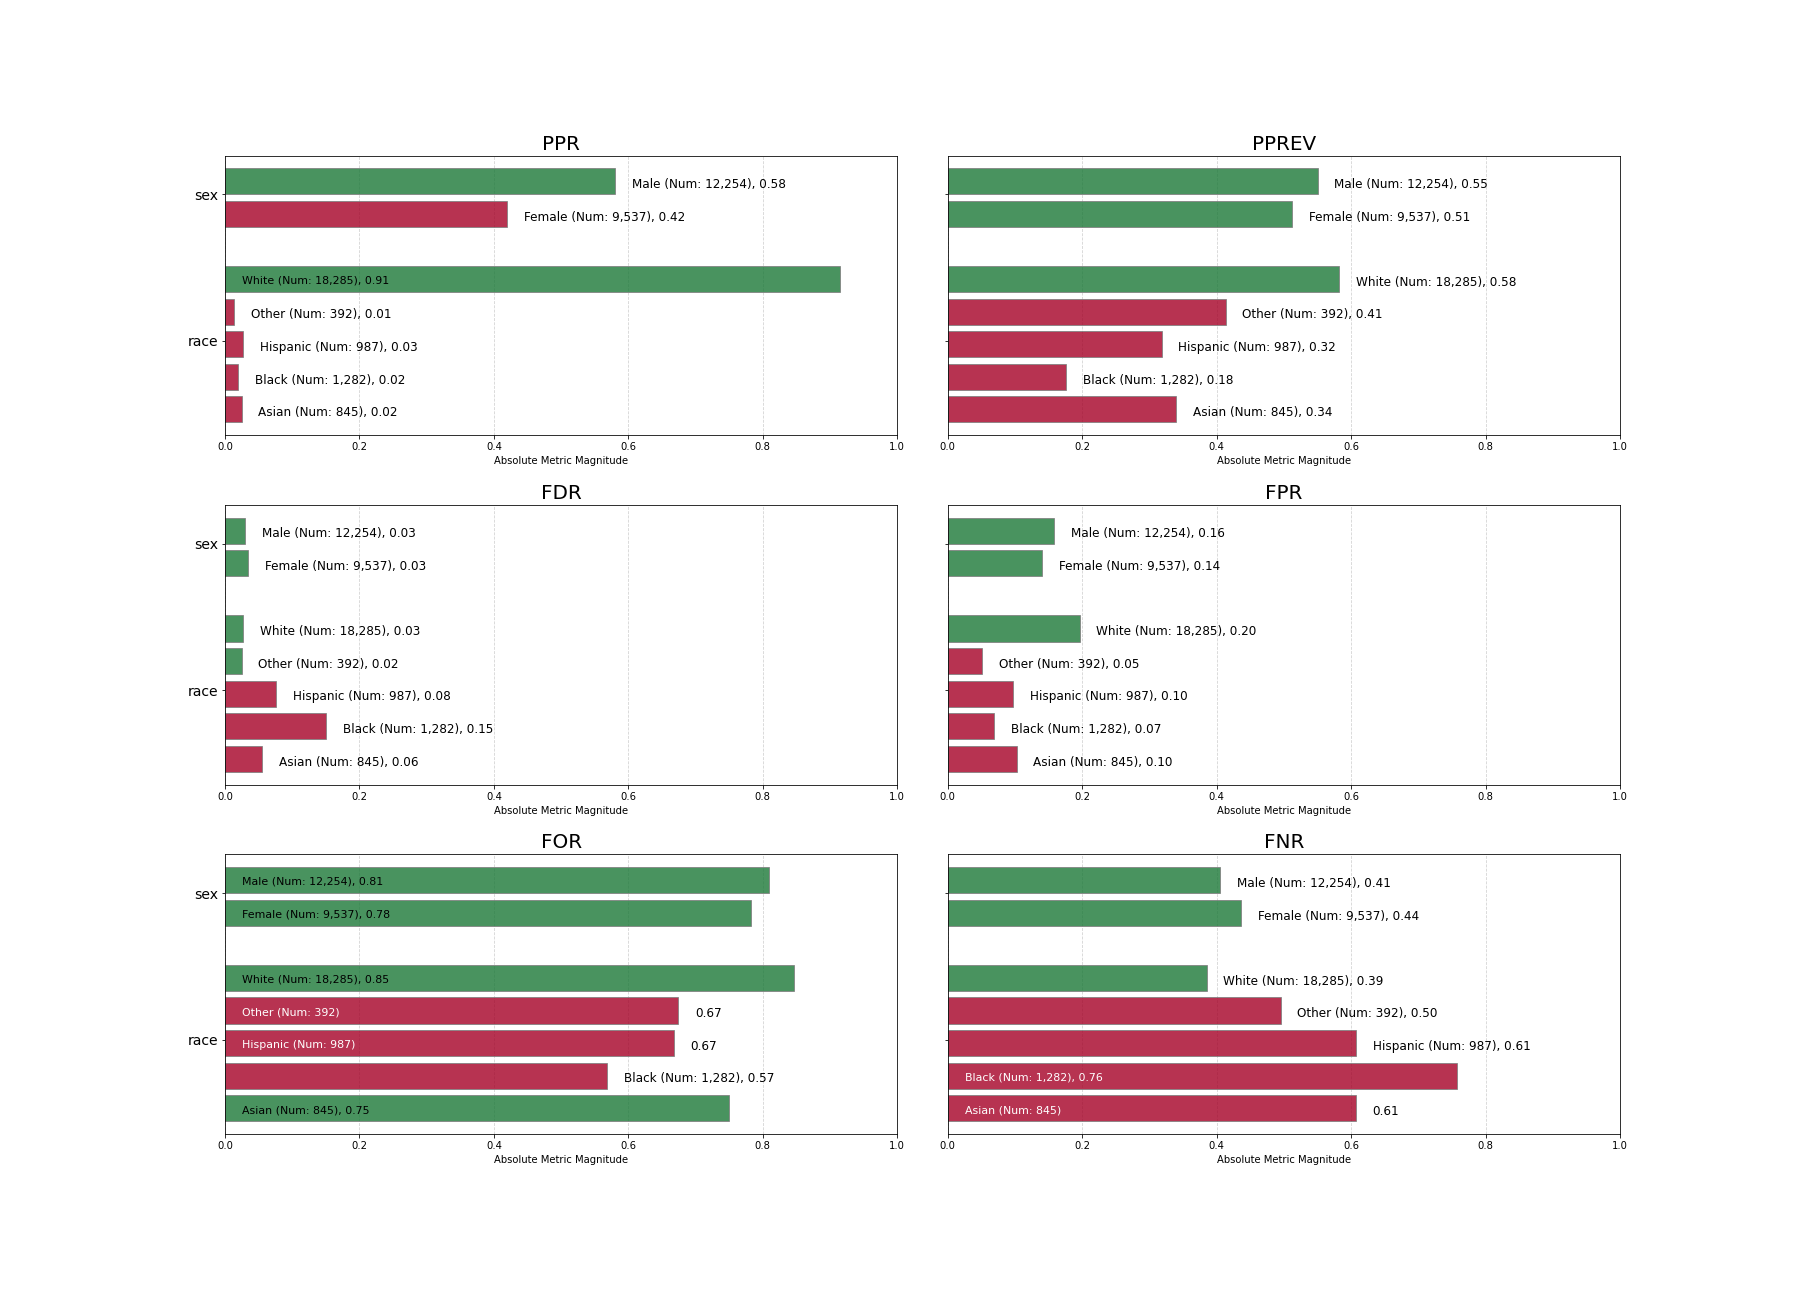
\includegraphics[width=21.3cm]{disparity_group_law.png}
	\caption{Resultado de las métricas de grupo para \textit{law\_data} con $\tau=0.8$.}
    \label{fig:lawdgroup}
\end{figure}

\clearpage

Observando la Figura \ref{fig:lawdisparity} podemos ver que el conjunto de datos \textit{law\_data} no es justo para ninguna de las métricas para el atributo raza, siendo la FNR para los individuos de raza negra casi el doble que para los de raza blanca y 1.5 veces mayor para el resto de razas. La tasa de falsos negativos (FNR) nos dice que los individuos de cualquier raza tienen casi entre un 1.5-2 veces más de probabilidad de ser etiquetados con notas bajas, cuando realmente obtendrían una mejor calificación. Esto hace evidente la existencia de un problema de sesgo para esta métrica.  En cuanto al sexo, los resultados son justos para ambas métricas. Esto nos puede dar la idea de que en este problema, no existe un sesgo determinante para el sexo, conclusión que ya obtuvimos en la Sección \ref{sec:contrastresults}.\\

\begin{figure}[h]
	\hspace{-2.5cm}
	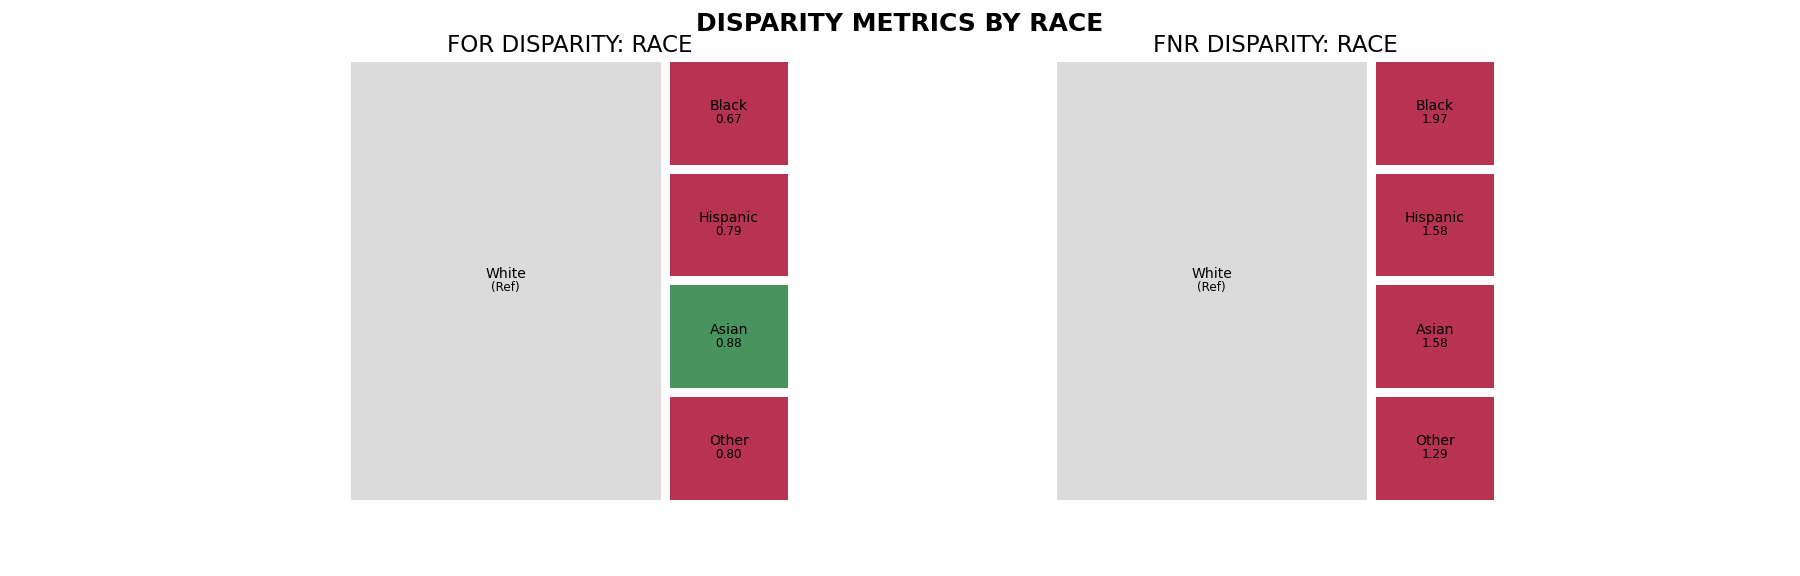
\includegraphics[width=21.3cm]{images/disparity_law_race.png}
	
	\hspace{-2.5cm}
	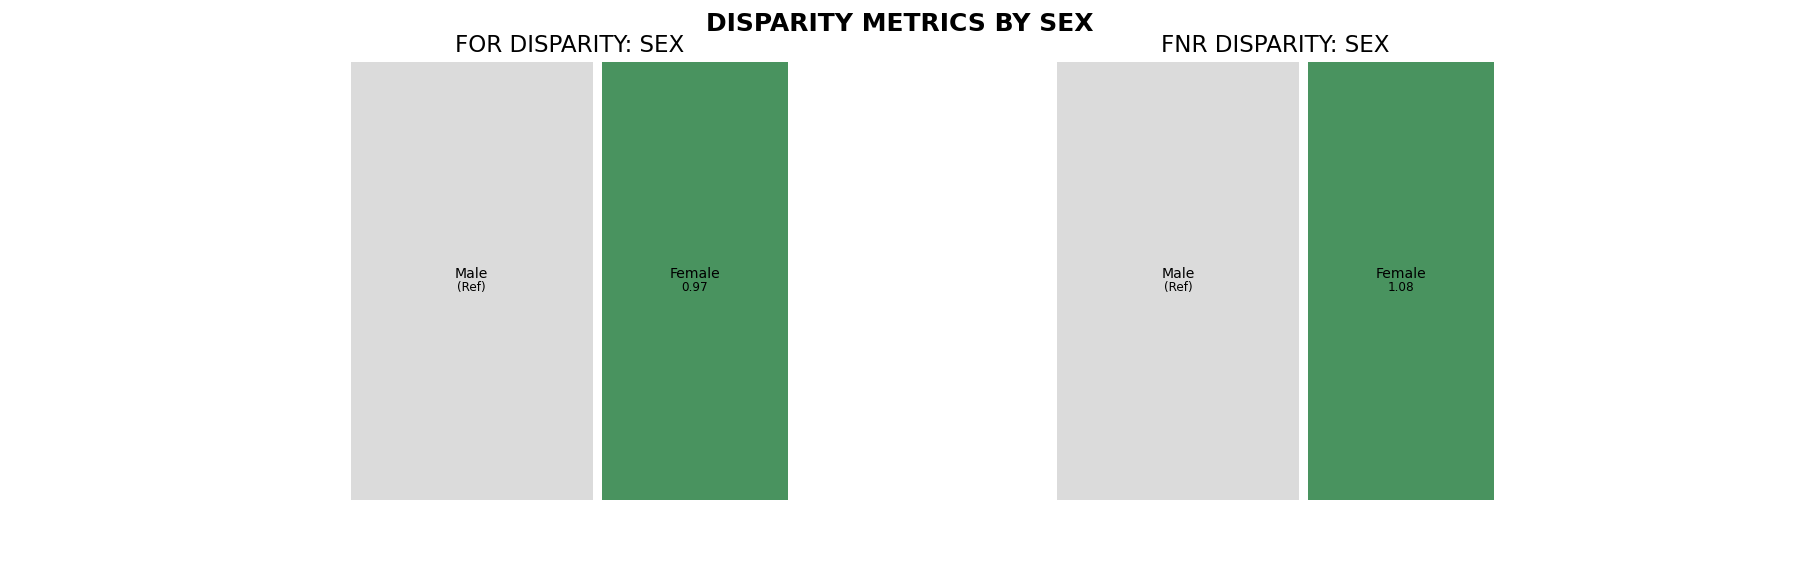
\includegraphics[width=21.3cm]{images/disparity_law_sex.png}
	\caption{Resultado de las métricas de disparidad para \textit{law\_data} con $\tau=0.8$.}
    \label{fig:lawdisparity}
\end{figure}